\documentclass[acmsmall,screen,review]{acmart}
\usepackage{algorithm}
\usepackage{algpseudocode}
\usepackage{booktabs}
\usepackage{multirow}
\usepackage{listings}
\usepackage{xcolor}
\usepackage{amsmath}
\usepackage[capitalize]{cleveref}
\usepackage{xspace}
\usepackage{xurl}
\usepackage{tikz}
\usetikzlibrary{arrows.meta,positioning,shapes.geometric}
\newcommand{\tool}{\textsc{kfold}\xspace}

\AtBeginDocument{%
  \providecommand\BibTeX{{Bib\TeX}}}

\setcopyright{none}
\settopmatter{printacmref=false}

\lstset{
  basicstyle=\ttfamily\footnotesize,
  keywordstyle=\bfseries\color{blue!70!black},
  commentstyle=\itshape\color{green!50!black},
  stringstyle=\color{red!60!black},
  breaklines=true,
  numbers=left,
  numberstyle=\tiny\color{gray},
  stepnumber=1,
  numbersep=5pt,
  frame=single,
  tabsize=2
}

\begin{document}

\title{\tool: Guarded Object Selection Conditions for Kbuild Makefiles}

\author{Anonymous Author(s)}
\affiliation{%
  \institution{Anonymous Institution}
  \country{USA}
}

\begin{abstract}
Configurable systems use Kbuild Makefiles to decide which objects participate in a build. Running Make under one configuration reveals one selection, but does not describe the conditions for other selections. We present \tool, an analyzer that extracts approximate, Kbuild-local object-selection conditions from a supported subset of GNU Make. It represents alternative variable words with Boolean guards and merges conditional effects after each branch. The resulting conditions retain information about assignments, composite objects, and directory reachability without enumerating a state for every branch combination.

We study five systems and compare extracted conditions with local GNU Make expansion and observed object files. In four Linux configurations, precision against physical objects ranges from 87.7\% to 99.1\%; almost every observed object within the analyzer's target set is predicted. However, only 33.7--44.4\% of all observed physical object paths overlap those predictions. Barebox agrees on 376 of 393 predictions, while U-Boot misses 12 objects within its target set and omits 231 observed paths from that set. These results support guarded analysis of common Kbuild selections but do not establish a complete build map. The conditions omit Kconfig dependencies, and satisfying assignments have not been validated as buildable configurations.
\end{abstract}

\begin{CCSXML}
<ccs2012><concept><concept_id>10011007.10011074.10011099.10011692</concept_id><concept_desc>Software and its engineering~Software verification</concept_desc><concept_significance>500</concept_significance></concept></ccs2012>
\end{CCSXML}
\ccsdesc[500]{Software and its engineering~Software verification}
\keywords{Kbuild, build systems, variability, symbolic execution, object selection}
\maketitle
\pagestyle{plain}

\section{Introduction}
\label{sec:intro}

The build system determines which source files reach the compiler. In the Linux kernel and related projects, Kbuild expresses this choice through Make variables such as \texttt{obj-\$(CONFIG\_USB)} and through conditionally selected subdirectories. A concrete build reveals the objects selected by one \texttt{.config}; it cannot by itself answer which option settings would select a different object. A build-level selection condition could help explain a missed source file, compare build rules across releases, or guide a search for a configuration that enables a target. The last use also requires the independent constraints in Kconfig and confirmation by the project's configurator.

Recovering such conditions requires more than finding \texttt{CONFIG\_*} strings. Make evaluates some right-hand sides immediately and others when referenced. An assignment can have a configuration-dependent variable name, so an overwrite may affect \texttt{obj-y} in one configuration and a different variable in another. A file selected in a subdirectory also inherits the condition under which its parent enters that directory. Composite targets add another layer between an object listed in \texttt{obj-y} and the source objects that contribute to it.

Prior work established static extraction of Kbuild configuration information: \textsc{Kmax} identifies build constraints~\cite{kmax,gazzillo2018localizing}, and Nguyen and Nguyen studied symbolic execution of Kbuild Makefiles~\cite{nguyen2020kbuild}. Our question is how a guarded-value implementation handles computed assignment names, branch joins, composite objects, and repeated directory reachability as one object-condition pipeline, and where that pipeline stops matching physical builds. We merge branch effects at statement boundaries instead of retaining an environment for every completed branch combination. Guarded words and their formulas can still grow sharply.

\tool evaluates a supported Kbuild subset and associates each extracted object with a formula over the configuration values it observes. We call this a \emph{Kbuild-local object-selection condition}: it describes the tool's interpretation of Makefile selection. It is neither a proof of compilation nor a configuration accepted by Kconfig.

Across four Linux configurations, 87.7--99.1\% of predicted physical object paths appear in the corresponding inventories, but the predictions overlap only 33.7--44.4\% of all observed paths. On the non-Linux subjects, a missing top-level U-Boot selection accounts for 12 observed objects inside the analyzer's target set. These results locate both useful agreement and an entry-point boundary; they do not turn the extracted formulas into a complete build map.

Our contributions are:
\begin{enumerate}
\item An implementation of guarded variable values, conditional merging, guarded overwrites, composite-object expansion, and conditional directory traversal for Kbuild-style Makefiles (\Cref{sec:design}).
\item An empirical comparison with GNU Make and compiler-produced objects, including a correction to the configuration valuation used for Barebox and Das U-Boot and an explicit accounting of observed objects outside the extracted target set (\Cref{sec:eval}).
\item A characterization of the current boundary: construct frequency, runtime, comparison scope with \textsc{Kmax}, and the limits imposed by missing Kconfig constraints and unsupported Make behavior (\Cref{sec:eval,sec:discussion}).
\end{enumerate}

\section{Overview}
\label{sec:overview}

\Cref{fig:pipeline} follows the input from Kbuild files and project entry points through relevant statements, guarded values, and directory conditions to a formula for each extracted object path. The figure separates this symbolic result from a later comparison with a normalized configuration and observed objects. We next follow one file through these stages before giving the algorithm in \Cref{sec:design}.

\begin{figure*}[t]
\centering
\resizebox{\textwidth}{!}{%
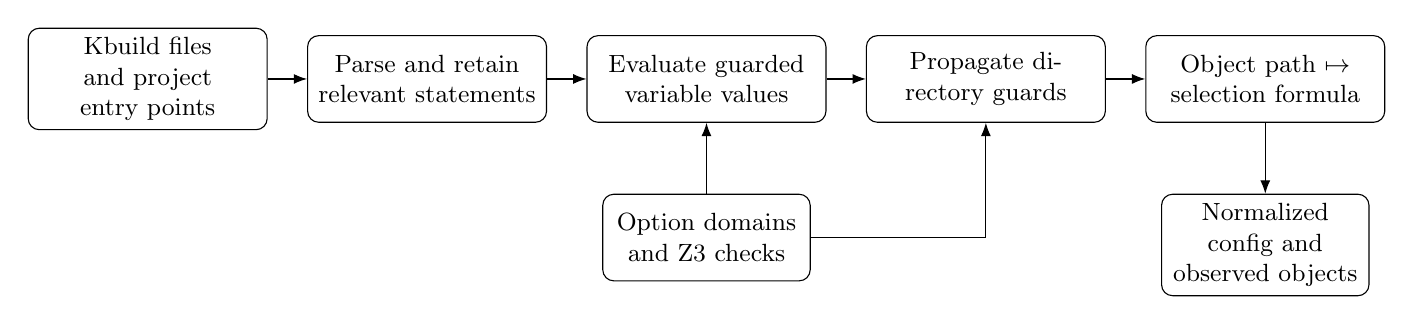
\begin{tikzpicture}[>=Latex, node distance=5mm and 5mm,
  box/.style={draw,rounded corners,align=center,minimum height=11mm,text width=28mm,font=\small},
  smallbox/.style={draw,rounded corners,align=center,minimum height=11mm,text width=24mm,font=\small}]
\node[box] (source) {Kbuild files and project entry points};
\node[box,right=of source] (parse) {Parse and retain relevant statements};
\node[box,right=of parse] (execute) {Evaluate guarded variable values};
\node[box,right=of execute] (walk) {Propagate directory guards};
\node[box,right=of walk] (output) {Object path $\mapsto$ selection formula};
\draw[->] (source)--(parse);\draw[->] (parse)--(execute);\draw[->] (execute)--(walk);\draw[->] (walk)--(output);
\node[smallbox,below=9mm of execute] (domain) {Option domains and Z3 checks};
\draw[->] (domain)--(execute);\draw[->] (domain)-|(walk);
\node[smallbox,below=9mm of output] (concrete) {Normalized config and observed objects};
\draw[->] (output)--(concrete);
\end{tikzpicture}}
\caption{The analysis produces Kbuild-local selection formulas before any concrete comparison. Configuration normalization and physical object inventory are separate validation inputs, not steps that make the symbolic conditions valid Kconfig assignments.}
\Description{A five-stage flow from Kbuild files and entry points through parsing, guarded-value evaluation, conditional directory traversal, and object selection formulas. Option domains feed evaluation and traversal; a normalized configuration and observed objects enter only after extraction.}
\label{fig:pipeline}
\end{figure*}

\subsection{Kbuild selection in brief}
Kbuild uses GNU Make variables to describe objects. A line such as \texttt{obj-\$(CONFIG\_NET) += net.o} computes the destination variable name from an option. If the option expands to \texttt{y}, the word is appended to \texttt{obj-y}; \texttt{m} selects \texttt{obj-m} where modules are relevant; an unset value commonly produces \texttt{obj-}, which is not selected as a normal target. A directory word ending in \texttt{/} asks Kbuild to descend into another Makefile. A target such as \texttt{driver.o} may itself be assembled from \texttt{driver-objs}, \texttt{driver-y}, or other project-specific lists. The file therefore carries both a local selection condition and a reachability condition inherited from its parents.

GNU Make also distinguishes immediate assignment with \texttt{:=} from deferred assignment with \texttt{=}. The former expands its right-hand side at assignment time. The latter retains an expression that can depend on subsequent variable updates. \texttt{+=} follows the variable's existing flavor; \texttt{?=} only assigns when the variable is undefined. These details affect target words even when the Makefile contains no explicit conditional directive. A static scan for \texttt{CONFIG\_*} names cannot recover the resulting selection formula because it does not know which assignment wins, when a reference expands, or whether a parent directory is entered.


Our input is a source tree, its project-specific \texttt{skbuild.ini} entry-point and target-variable settings when present, and a choice of Boolean or tristate option domain. The main output is a set of object paths with formulas over those options. A later evaluator substitutes a normalized \texttt{.config} into the formulas; the symbolic analysis itself does not invoke recipes or compile code. The implementation parses Make syntax using \texttt{pymake3}, evaluates a supported subset, and uses Z3 for condition checks. It uses a map from words to formulas, which combines duplicate words and loses their order. This representation is useful for set-valued object selection and is not a general replacement for GNU Make's ordered strings.


\Cref{lst:example} is a simplified Kbuild example. It combines an assignment to a computed variable name, an overwrite, a conditional branch, and a composite target. Assume for this example that the named options have values \texttt{y} or unset. The desired output is a condition for each object, rather than a list for one chosen configuration.

\begin{lstlisting}[language=make,float=t,caption={Simplified Kbuild example. The final object conditions also depend on the guard under which this directory is entered.},label={lst:example}]
obj-$(CONFIG_NET) += net_core.o
obj-$(CONFIG_FAST) := fast_net.o
ifeq ($(CONFIG_WIDE),y)
  WIDTH := 64
else
  WIDTH := 32
endif
obj-y += driver_$(WIDTH).o
fast_net-y += accelerator.o
\end{lstlisting}

First, \texttt{net\_core.o} enters \texttt{obj-y} when \texttt{CONFIG\_NET=y}. The second statement overwrites \texttt{obj-y} when \texttt{CONFIG\_FAST=y}. Consequently the surviving local condition for \texttt{net\_core.o} is \texttt{CONFIG\_NET=y} $\land$ \texttt{CONFIG\_FAST}$\ne$\texttt{y}, while \texttt{fast\_net.o} has local condition \texttt{CONFIG\_FAST=y}. The branch gives \texttt{WIDTH} guarded alternatives \texttt{64} and \texttt{32}; the later append gives \texttt{driver\_64.o} condition \texttt{CONFIG\_WIDE=y} and \texttt{driver\_32.o} its negation. Because \texttt{fast\_net.o} is composite, its member \texttt{accelerator.o} also depends on the selection of that parent object.

\tool stores these alternatives as words paired with conditions. It evaluates the two sides of the \texttt{ifeq} using copies of the current state, combines the resulting guarded values at \texttt{endif}, and continues with one merged environment. Finally it combines local object conditions with the condition for reaching the directory. The example describes the intended data flow; the evaluation tests agreement with actual builds, where Make conventions and generated rules are more varied.


\subsection{A trace from assignments to object conditions}
\label{sec:overview:trace}
\Cref{tab:example-trace} records the state changes in \Cref{lst:example}. We write $N$ for \texttt{CONFIG\_NET=y}, $F$ for \texttt{CONFIG\_FAST=y}, and $W$ for \texttt{CONFIG\_WIDE=y}. The first row is easy: one word has guard $N$. The second is the point where a text-oriented analysis can fail. The assignment destination is \texttt{obj-y} only when $F$ holds, so a previous word survives when $\neg F$ holds. A global overwrite of \texttt{obj-y} would lose \texttt{net\_core.o}; ignoring the overwrite would retain it under $N\land F$ even though Make has replaced the value in that configuration.

\begin{table}[t]
\centering\footnotesize
\caption{Selected guarded words after each statement of \Cref{lst:example}. The final column assumes this directory is reached under guard $D$. The map records membership, not word order or multiplicity.}
\label{tab:example-trace}
\begin{tabular}{lll}
\toprule
Step & State change & Final selection contribution \\
\midrule
First append & \texttt{net\_core.o}: $N$ & $D\land N\land\neg F$ \\
Overwrite & \texttt{fast\_net.o}: $F$ & $D\land F$ \\
Conditional & \texttt{WIDTH}: $64$ under $W$, $32$ under $\neg W$ & --- \\
Later append & \texttt{driver\_64.o}: $W$ & $D\land W$ \\
Later append & \texttt{driver\_32.o}: $\neg W$ & $D\land\neg W$ \\
Composite & \texttt{accelerator.o} belongs to \texttt{fast\_net.o} & $D\land F$ \\
\bottomrule
\end{tabular}
\end{table}

The conditional assignment to \texttt{WIDTH} forks the state just long enough to execute each arm. At the join, the two values are retained as guarded alternatives. Expanding \texttt{driver\_\$(WIDTH).o} then yields two different words with complementary guards. The last line of the example describes a composite: the parent \texttt{fast\_net.o} is selected under $F$, so its unconditional member \texttt{accelerator.o} inherits $F$. All of these local conditions are conjoined with the guard $D$ under which the directory is reached. This is the end-to-end result the tool reports for the example, not a claim that the configuration assignments satisfy an external Kconfig specification.

The value map is compact when many branches change different variables, because alternatives live inside values instead of a retained environment for every branch combination. It can still grow sharply. A variable name assembled from several guarded fragments can create a cross-product of alternatives; formulas may also become expensive to simplify. The implementation bounds one such expansion and uses approximations in other cases. We therefore describe branch merging as a representation choice and measure observed runtime separately, rather than claiming asymptotic immunity to path explosion.

\subsection{The same object through two directories}
\label{sec:overview:directories}
Suppose a root Makefile selects \texttt{a/} under option $A$ and \texttt{b/} under option $B$, and both directories select \texttt{shared/}. If \texttt{shared/Makefile} selects \texttt{x.o}, the path condition for \texttt{x.o} is $A\lor B$. Marking \texttt{shared/} simply ``visited'' after the $A$ path would lose the $B$ contribution. The analyzer instead stores, for each Makefile, the disjunction of conditions already propagated to it. When $B$ arrives, it processes only $B\land\neg A$; if $B$ is already covered by $A$, it does no new work. A back edge from \texttt{shared/} to \texttt{a/} consequently stops when it contributes no new configuration. This example explains why directory traversal is a conditional worklist rather than a depth-first walk with a Boolean visited flag.

\section{Technique}
\label{sec:design}

\subsection{Selection model and algorithm}
A configurable build has at least three distinct decisions. A configurator decides which assignments are permitted and normalizes a user's proposed settings. A build description maps those settings to targets and directories. Finally, recipes and compiler invocations turn selected targets into physical artifacts. These stages are related, but they are not interchangeable. A condition extracted from a Makefile answers a question about the second stage under the analyzer's interpretation of Make. It does not, by itself, show that Kconfig permits the assignment or that a compiler can build the selected source.

Let $M$ be a collection of Kbuild Makefiles and $c$ an assignment to the option symbols used by those files. For an object path $o$, write $S_M(o,c)$ when evaluating the supported Kbuild selection rules under $c$ selects $o$. The analysis aims to produce a formula $\Phi_M(o)$ such that evaluating $\Phi_M(o)$ under a concrete $c$ predicts this selection. The implemented formula is an \emph{approximation} of $S_M$: the supported language is narrower than GNU Make, and the entry points configured for a project may omit top-level orchestration. We use $\Phi_M$ as a queryable explanation of a modeled selection, not as a statement of whole-build equivalence.

The distinction matters for every proposed use. A formula $\Phi_M(o)$ may be satisfiable even though Kconfig rejects its model. An observed \texttt{.o} may have no $\Phi_M(o)$ because it is a generated or intermediate target or because the relevant directory was outside the traversal. Conversely, a selected object may not appear on disk because a later build stage did not run, failed, or reused an artifact. The evaluation records these cases separately rather than treating one set of paths as a complete oracle for another.


For one parsed Makefile, the executor maps each variable name to guarded words. An entry $w\mapsto\phi$ says that word $w$ is present under option condition $\phi$ in the modeled state. The run begins at configured Makefile entry points $E$ and uses project settings $\Gamma$ for target families and option domains. Its output is a map from object paths to formulas, not a claim about whether Kconfig accepts a valuation or a compiler emits an object.

\Cref{alg:extract} gives the end-to-end procedure. Lines 3--8 admit only a satisfiable part of an incoming directory guard that has not reached the same file before. Lines 9--13 parse, reduce, and execute a file once, restrict its cached state to that new guard, and record the resulting instance. Lines 14--16 queue selected child directories. After the queue empties, lines 18--24 extract target and composite-member paths from the restricted instances and disjoin repeated contributions. The runner persists those instances; the extraction interface performs the last aggregation. A missing entry file contributes no edge, and a parse or execution error can stop a run rather than produce a complete map.

\begin{algorithm}[t]
\caption{Extract guarded Kbuild-local object conditions}
\label{alg:extract}
\begin{algorithmic}[1]
\Require source tree $M$, entry files $E$, project settings $\Gamma$
\Ensure object-path map $\Phi$, or an analysis error
\State $R[m]\gets\bot$ for each file $m$; $Q\gets\{(e,\top):e\in E\}$
\State $C\gets\emptyset$; $I\gets\emptyset$
\While{$Q$ is nonempty}
  \State remove $(m,\gamma)$ from $Q$
  \State $\delta\gets\gamma\land\neg R[m]$
  \If{$\delta$ is unsatisfiable}
    \State \textbf{continue}
  \EndIf
  \If{$m\notin C$}
    \State $C[m]\gets\operatorname{execute}(\operatorname{reduce}(\operatorname{parse}(m)),\Gamma)$
  \EndIf
  \State $S\gets\operatorname{restrict}(C[m],\delta)$
  \State $R[m]\gets R[m]\lor\gamma$; add $S$ to $I$
  \For{each selected directory $(d,\eta)$ in $S$}
    \State add $(\operatorname{entry}(d),\eta)$ to $Q$ if its file exists
  \EndFor
\EndWhile
\State $\Phi\gets\emptyset$
\For{each restricted instance $S\in I$}
  \For{each path and guard $(o,\phi)\in\operatorname{targets}(S,\Gamma)$}
    \State $\Phi[o]\gets\Phi[o]\lor\phi$ (initially $\bot$)
  \EndFor
\EndFor
\State \Return $\Phi$
\end{algorithmic}
\end{algorithm}

The finite set of source files and finite option domains make $R[m]$ monotone over a finite set of valuations. The worklist stops when every pending guard is already covered or unsatisfiable. This prevents a directory back edge from causing an infinite revisit under the same condition. It does not supply targets missing from the configured entry graph. In the overview example, $C[m]$ contains the two guarded \texttt{WIDTH} words; restricting that state by parent condition $D$ produces $D\land W$ and $D\land\neg W$ before target extraction. The shared-directory example contributes $A$ and then $B\land\neg A$, yielding $A\lor B$ for \texttt{x.o}.

\subsection{State and observation unit}
The observation unit is deliberately a path, not a source file. An object path can denote a compiler output, a composite link target, a generated object, or an intermediate object. The analyzer's target records primarily come from configured target-variable families and selected composite lists. This choice makes object selection queryable, but it does not equate every reported path with one compilation unit. The physical comparisons in \Cref{sec:eval} use the same path spelling only where a mapping is justified.

The word map is a material approximation. GNU Make variables are strings whose ordering, repeated words, and whitespace can affect later functions. A keyed map collapses duplicate words and does not preserve their sequence. For membership in an \texttt{obj-y} list this collapse is often harmless; for \texttt{firstword}, \texttt{wordlist}, or a macro that depends on position it can be wrong. We therefore describe the implementation as a selection analyzer for a Kbuild subset, not as a GNU Make interpreter. The construct census measures syntax encountered, and concrete comparisons probe consequences of these approximations.

\subsection{Preprocessing and dependence reduction}
The implementation reads a Makefile, normalizes line endings, parses it with \texttt{pymake3}, and performs a preliminary dependency pass. That pass identifies variables that may influence target families and removes statements deemed irrelevant to target extraction. The symbolic pass then executes the reduced statement list against a fresh guarded state. This two-pass arrangement is useful because production Makefiles contain flags, recipes, and other definitions not needed for object-list membership. It is also a possible source of underapproximation: a dependency missed by the preliminary pass may cause a statement that matters to be removed.

The parser maps assignments, condition blocks, rules, commands, includes, and several directives to internal statement classes. Assignment and condition classes have symbolic execution behavior. Rules and recipes are eliminated from the target-selection pass; their effects on generated prerequisites and later Make execution are outside this model. Include directives are parsed and counted, but the current symbolic execution method for them is a no-op. This matters whenever an included fragment defines a target list that the containing Makefile does not repeat. Similarly, a Makefile included at top level does not become reachable merely because the tool analyzes a child directory. On a file-read error, preprocessing logs a warning and parses empty text; this can yield an incomplete map without stopping the run.

\subsection{Guarded assignment and variable flavor}
Consider an assignment whose left-hand side expands to name $x$ under guard $\psi$. An append adds each expanded right-hand word under the conjunction of $\psi$ and the word's own expansion guard. An overwrite replaces the value of $x$ where $\psi$ holds, while an old word guarded by $\phi$ survives under $\phi\land\neg\psi$. If an old and a new contribution have the same word, their guards are disjoined. This is the key operation behind the overwrite in \Cref{sec:overview:trace}. It also applies when the conditional behavior comes from the computed \emph{name} rather than an explicit \texttt{ifeq}.

The executor records immediate and recursive flavors. For \texttt{:=}, it expands the right-hand side during assignment; for \texttt{=}, it stores text to be expanded when the value is referenced. GNU Make's \texttt{+=} follows the existing variable's flavor, while this symbolic execution path expands the appended right-hand side immediately. The implementation has separate handling for \texttt{?=} and recognizes \texttt{::=}, but the internal overwrite predicate treats only \texttt{=} and \texttt{:=} as ordinary replacements of an existing value. Consequently the current behavior for all flavor combinations should not be read as a verified implementation of GNU Make. A deferred value can also interact with a later symbolic update in ways that the word-map abstraction does not fully preserve. We isolate these semantics as a conformance gap rather than claiming that the observed build agreement validates each assignment operator.

\begin{table}[t]
\centering\footnotesize
\caption{Selected Make constructs and the interpretation used in this study. ``Parsed'' means that syntax is recognized; it does not imply faithful GNU Make behavior.}
\label{tab:scope}
\begin{tabular}{p{25mm}p{43mm}p{56mm}}
\toprule
Construct & Implemented path & Material boundary \\
\midrule
\texttt{+=}, \texttt{=}, \texttt{:=} & Guarded words and variable flavor & Append expands immediately; order and duplicates are lost. \\
\texttt{?=}, \texttt{::=} & Parsed; partial assignment handling & Existing-value and flavor cases need differential checks. \\
\texttt{ifeq}, \texttt{ifneq}, \texttt{ifdef}, \texttt{ifndef} & Clone arms, execute, re-guard, merge & Expansion approximations enter condition tests. \\
Text functions and \texttt{call} & Symbolic alternatives for common cases & Cross-products may be bounded or collapsed. \\
\texttt{include} & Parsed and counted & Included statements are not symbolically executed. \\
Rules and recipes & Removed from selection pass & Generated and side-effecting behavior omitted. \\
\texttt{\$(shell ...)} & Concrete subprocess invocation & Host environment may affect results. \\
\bottomrule
\end{tabular}
\end{table}

\subsection{Conditional execution and branch merge}
A condition evaluator expands the two sides of \texttt{ifeq} or \texttt{ifneq} into guarded alternatives. Equality holds under the disjunction of compatible pairs of alternative guards. For \texttt{ifdef} and \texttt{ifndef}, the evaluator checks whether the selected variable's expansion is undefined under each guard. A multi-arm \texttt{else ifeq} is represented as a nested conditional in the remaining else arm, so only the first matching arm contributes.

At a condition block, the executor clones the entering state for the then and else arms and executes each clone under its branch guard. At the join it rebuilds only variables touched in either arm. If an entry $w$ has guard $\phi_t$ in the then state and $\phi_e$ in the else state, the merged guard is $(\psi\land\phi_t)\lor(\neg\psi\land\phi_e)$, with the ambient parent condition included in both branch guards. Re-guarding is necessary even for a word carried through a branch without being touched: otherwise a value overwritten in one arm can reappear through the other arm's unguarded carry-over. Untouched variables keep their entering representation, limiting needless formula growth.

The join leaves one state at the following statement boundary. It does not make memory constant. A single variable may have many guarded alternatives; name and value expansions can multiply alternatives; and Z3 formulas can grow or require expensive satisfiability checks. An old synthetic fork-per-branch benchmark illustrates the motivation for merging, but it is not a fair full-tool baseline and is not used as the primary scalability claim in this paper. The empirical timing results describe the implementation as a whole under the stated workload.

\subsection{Computed names and expansion functions}
In \texttt{obj-\$(CONFIG\_X) += foo.o}, the left-hand expression can produce \texttt{obj-y}, \texttt{obj-m}, or an unselected variable name under distinct guards. The executor expands the name before updating state, then combines the name guard, ambient branch guard, and value guard. This is why a single Makefile assignment can produce several target-family contributions. The same mechanism applies to computed words such as \texttt{driver\_\$(WIDTH).o} in the overview.

The expansion layer recognizes variable references and a range of text functions, including substitution, filtering, prefix and suffix addition, string tests, positional words, \texttt{foreach}, and \texttt{call}. Its implementation is intentionally bounded: when a concatenation creates more than 64 alternatives, it collapses them to one joined string under an unconditional guard. This prevents some combinatorial blow-ups but can lose correlations and produce incorrect target words. A function that is recognized and counted in the census may therefore still be approximate for a particular use. Unsupported substitution references are recorded separately.

A \texttt{\$(shell ...)} expression is handled by launching a concrete subprocess with a five-second timeout and using its output. Thus an analysis may depend on the host shell, tools, filesystem, and command exit behavior. The main object-selection algorithm does not run Make recipes or compile targets, but it is not a fully hermetic or side-effect-free parser. The current artifact does not log every such command and result in the experiment manifest. Reproducibility and security assessments need to account for this execution path.

\subsection{Conditional directory reachability}
\label{sec:design:worklist}
The starting set is an explicit Makefile, the project-configured top directories, or a fallback discovery set when those entry points yield no files. For a Makefile reached under $\rho$, its local state is restricted by $\rho$; directory words in relevant target variables produce child paths and guards. If two parents select the same child, the child receives the disjunction of incoming conditions. Paths are resolved to canonical filesystem paths so a syntactic \texttt{../} back edge refers to the same Makefile.

A Boolean visited set is unsound for a shared child: the first visit may cover $A$ while a later path adds $B$. The implementation maintains $R[m]$, the union of conditions already propagated for Makefile $m$. For an incoming guard $\gamma$, it computes $\delta=\gamma\land\neg R[m]$. If $\delta$ is unsatisfiable, the visit is skipped. Otherwise the file's cached local analysis is restricted by $\delta$, its targets and descendants receive that condition, and $R[m]$ becomes $R[m]\lor\gamma$. This is a monotone worklist over the modeled option domain. A cycle that adds no new configuration is skipped, while a genuinely broader route still propagates. The procedure addresses infinite revisits caused by directory cycles; it does not add selection rules absent from the chosen entry points.



\subsection{Target families, composites, and aggregation}
\label{sec:design:targets}
The project settings specify target-variable prefixes. Conventional Kbuild uses \texttt{obj-} and \texttt{lib-}; Barebox and coreboot require additional families for preboot or firmware stages. The extractor ignores unselected suffixes and records target words ending in \texttt{.o} or \texttt{.a}; some dialect mappings also translate source suffixes to object paths. Composite resolution follows definitions such as \texttt{target-objs}, \texttt{target-y}, and \texttt{target-m}. A member inherits the conjunction of its own condition and its selected parent target's condition. When the same object path is reached through several analyzed instances, their conditions are disjoined.

This path aggregation is a set operation. It does not retain the multiplicity or order of link inputs. It also does not guarantee that every compiler-produced \texttt{.o} has a corresponding extracted path. The physical inventory includes generic \texttt{built-in.o} intermediates, architecture outputs, generated files, and outputs from rules outside the target families. In coreboot, one source path can produce stage-specific artifacts, so the mapping must include a stage prefix. These differences motivate the explicit outside-universe counts in the evaluation rather than silently dropping unmatched objects.

\subsection{Interpreting a formula}
A reported formula ranges over the symbolic option values modeled by this run. In a Boolean run the default option domain contains \texttt{y} and unset; in a tristate run it also contains \texttt{m}. Some project settings add finite domains for other names. Z3 checks whether guards are satisfiable in that local domain. The solver does not know Kconfig's \texttt{depends on}, \texttt{select}, choice, and normalization rules. A satisfying assignment is therefore a candidate input for a configurator, not a buildable witness.

The experimental evaluator substitutes values from a normalized \texttt{.config} into \emph{every option variable appearing in each target formula}. This detail is material: the earlier validation code looked only at option names in an auxiliary state map and left many target conditions symbolic. The corrected comparisons in \Cref{sec:eval} use the formula variables themselves. They still inherit all limits of the extractor, entry-point settings, object mapping, and archived build status.

\section{Implementation and Measurement Interface}
\label{sec:implementation}

The implementation is organized around four persistent concepts. \texttt{Kbuild} owns parsing and symbolic execution of one Makefile. \texttt{DState} carries the preliminary dependency pass used to decide which statements can affect selected target-variable families. \texttt{SState} stores guarded words during the symbolic pass. \texttt{Run} discovers entry files, manages the directory worklist, caches per-file analysis, and records the restricted instances created by new reachability conditions. The distinction between a unique Makefile and an analyzed instance matters: a shared file can be loaded again under a newly arrived guard without being parsed from scratch, so instance count can exceed unique-file count. The Linux results report instances, while the cache in a run is keyed by canonical Makefile path.

A Boolean abstraction is insufficient for configurations with modules. Linux's evaluated Debian profile in our study contains 3,934 options assigned \texttt{m}. An initial two-value run predicted only 1,318 active target paths for that profile; the tristate rerun predicted 5,375. This large difference is one reason we distinguish the option domain used by an analysis from Kconfig's full rules. The tristate domain allows \texttt{y}, \texttt{m}, and unset; it does not encode all Kconfig dependencies, choices, or implicit assignments.


The solver layer represents option values with finite Z3 enumeration sorts. A project can use the default two-value domain or opt into the three-value domain that distinguishes \texttt{y}, \texttt{m}, and unset. The solver constructs equality conditions for option values and combines guards using conjunction, disjunction, and negation. Satisfiability queries are used in value restriction and reachability propagation. The solver's finite domains are an implementation of the local valuation space, not a Kconfig parser. Configurations used in the evaluation are normalized independently before they are substituted into formulas. The two-state versus tristate Linux discrepancy just reported illustrates why the choice of domain is part of the experiment protocol rather than a minor command-line preference.

A Makefile's local analyzed state is serialized into a per-run cache so that a later directory path can reuse it with a different incoming guard. The run output also records the settings and restricted Kbuild instances. The in-memory runner exposes conditions already propagated for each path and counts revisits skipped because they add no satisfiable configuration. These values make a directory cycle visible without imposing an arbitrary recursion-depth cutoff. They do not prove that the source tree has no other dynamic way to introduce a directory; only the recognized target words generate worklist edges.

The command-line and comparison scripts consume different views of this state. The corpus runner reports makefile instances, target records, construct counts, wall time, and process memory. The GNU Make comparison extracts local target-list words from each traversed file under a normalized configuration. The physical comparator instead walks archived object paths and evaluates the symbolic conditions, yielding $TP$, $FP$, $FN_U$, and $O$. These paths are kept as separate sets before percentages are computed. Keeping the full discrepancy lists in JSON allows a reviewer to reproduce a table entry or inspect a specific target without rerunning a large build.

There are two implementation caveats relevant to interpreting all subsequent measurements. First, the preliminary reduction and bounded string expansion are optimizations with semantic effects; neither has been exhaustively differential-tested against GNU Make for the corpora in this paper. Second, the concrete \texttt{\$(shell ...)} path can invoke host tools while analyzing a Makefile. A rerun may therefore depend on the same utilities and filesystem state even when its symbolic option domain is identical. The manifest records major tool versions and source hashes, but it is not a complete capture of every such host command. These caveats limit reproducibility and are not erased by agreement on a sampled physical build.

\section{Evaluation}
\label{sec:eval}

We evaluate three questions with different kinds of evidence. \emph{RQ1} asks how often formulas evaluated under a concrete configuration agree with locally expanded GNU Make target lists and with object files produced by builds. \emph{RQ2} asks how many Makefiles and target paths the implementation processes in the selected corpora, at what observed cost, and what can be learned from an archived \textsc{Kmax} comparison. \emph{RQ3} asks which construct categories occur in traversed files and which sources of disagreement remain visible. These questions do not collectively prove that an arbitrary reported formula is a faithful GNU Make condition or a Kconfig-feasible build condition.

\subsection{Subjects, configurations, and provenance}
\label{sec:eval:subjects}
The study uses BusyBox 1.36.1, coreboot 4.22.01, Barebox 2024.01.0, Das U-Boot 2024.01, and Linux v6.6 at commit \texttt{ffc253263a1375a65fa6c9f62a893e9767fbebfa}. The Linux analysis source has two local edits that add \texttt{-std=gnu11} to Makefile flags; their diff hash is recorded in the artifact manifest. The other source archive hashes are recorded where the archives remain available. A matching original coreboot archive was not found in the local cache, which limits exact replay of that subject. Project-specific \texttt{skbuild.ini} settings determine entry directories, target families, and exclusions.

\Cref{tab:profiles} separates a configuration used to value formulas from the status of its physical artifact inventory. Linux \texttt{tinyconfig} is an i386 build, while the other named Linux profiles use x86-64 paths. The normalized i386 tinyconfig and x86-64 defconfig clean GCC 12 rebuilds reproduced their archived sets exactly: 489 and 2,874 object paths. Barebox's fresh sandbox build likewise reproduced all 406 archived paths. U-Boot's fresh compilation produced all 1,123 archived objects plus 81 further paths, but final packaging failed because the Python \texttt{libfdt} module was unavailable; an EFI output-target workaround was also required. Debian and allmodconfig Linux comparisons reuse archives without a fresh build in this rerun. The coreboot QEMU i440fx archive was produced by an incomplete final ROM build. We retain these statuses because a partial build can make a predicted object look like a false positive.

\begin{table}[t]
\centering\footnotesize
\caption{Configuration and build provenance. ``Reproduced'' refers to equality of object-path sets with the archived inventory, not byte-identical object contents. A profile without a fresh build still has an archived object set used in the comparison.}
\label{tab:profiles}
\setlength{\tabcolsep}{3pt}
\begin{tabular}{p{22mm}p{33mm}p{36mm}p{35mm}}
\toprule
Subject & Configuration & Fresh build status & Archive status \\
\midrule
Linux & i386 tinyconfig & Completed with GCC 12 & 489 paths reproduced \\
Linux & x86-64 defconfig & Completed with GCC 12 & 2,874 paths reproduced \\
Linux & Debian x86-64 & Not rebuilt here & 15,419 archived paths \\
Linux & x86-64 allmodconfig & Not rebuilt here & 25,949 archived paths \\
Barebox & sandbox\_defconfig & Completed & 406 paths reproduced \\
U-Boot & sandbox\_defconfig & Compilation completed; packaging failed & 1,123 archived paths present \\
BusyBox & defconfig & Not rebuilt here & 191 archived paths \\
coreboot & QEMU i440fx & Not rebuilt here & 674 paths from partial ROM build \\
\bottomrule
\end{tabular}
\end{table}

Reruns used an Intel Core i7-7700 with eight logical CPUs and 31\,GiB of RAM on a Debian Linux host. The tool environment recorded Python 3.14.7, Z3 4.13.3, and GNU Make 4.4.1; clean Linux builds used GCC 12.5.0. The raw configuration hashes and source provenance are in \texttt{evidence/manifest.json}. All reported times are individual observed runs, not medians of repeated controlled trials. We therefore treat small timing differences as descriptive only. The main Linux traversal used the tristate domain; a two-state exploratory run is discussed only as a caution about option modeling.

\subsection{Comparison layers and denominators}
\label{sec:eval:method}
The analysis emits an extracted target-path set $U$ and a condition for each path. For a normalized configuration $c$, evaluating those conditions produces a predicted set $P_c\subseteq U$. The physical inventory $B_c$ is the set of archived \texttt{.o} paths after the comparison scripts' stated exclusions. Define $TP=|P_c\cap B_c|$, $FP=|P_c\setminus B_c|$, $FN_U=|(B_c\cap U)\setminus P_c|$, and $O=|B_c\setminus U|$. We report precision $TP/(TP+FP)$ and observed-path overlap $TP/|B_c|$. The restricted recall $TP/(TP+FN_U)$ is useful for checking valuations of \emph{recognized} paths, but excludes $O$ by definition and must not be described as whole-build recall. In this study restricted recall is near 100\% for most profiles even when overlap is near one third.

The $O$ group is heterogeneous. A generic \texttt{built-in.o} is a build intermediate that this target extractor intentionally omits. A path under an architecture tree may be produced by top-level orchestration outside the configured entry points. A stage-specific coreboot output can require a different path mapping from the source Makefile. Other paths can be genuine missed leaf targets. Thus $O$ is neither a count of semantic errors nor an ignorable residual. Likewise, $FP$ can include a selected target absent from a partial build, a composite target not emitted as a separate object in that build, or a wrong condition. The per-path JSON lists allow later classification, but the current study has not fully labeled every path.

The second comparison layer invokes GNU Make on each traversed Makefile with values from the same normalized configuration and reads the expanded target-list variables. It maps the resulting words to paths and intersects them with $U$. This is a \emph{local expansion} oracle for that file and variable set. It does not enforce directory reachability from the top-level build, and it does not reproduce all project-specific top-level variables or generated state. A local false negative therefore has a different interpretation from an object absent in a completed physical build. We report the two layers separately instead of averaging their precision and recall.

The corrected physical comparator extracts Z3 variables from each target formula, substitutes each corresponding configuration value, and disjoins conditions for duplicate target paths. The earlier archived script substituted only names visible in a side map of state variables. Most \texttt{CONFIG\_*} names occurred inside target formulas rather than that map, leaving them symbolic and causing the former very low Barebox and U-Boot recalls. This is an internal-validity correction to the measurement pipeline. The older result files remain in the repository for traceability but are not the source of the main tables.

\subsection{RQ1: Linux agreement across four profiles}
\label{sec:eval:linux}
\Cref{tab:linux-physical} reports the physical-path comparison. The predicted set grows from 185 paths for i386 tinyconfig to 11,615 for allmodconfig, which is expected because the latter enables many more built-in and modular selections. Precision is 95.1\%, 87.7\%, 98.2\%, and 99.1\% in profile order. Within the extracted target set there is no observed miss for three profiles; defconfig has one, \texttt{compat.o} under \texttt{security/keys/}. This restricted agreement should not obscure the larger inventory gap: only 33.7--44.4\% of all physical object paths overlap a prediction. The outside group ranges from 313 paths on tinyconfig to 14,436 on allmodconfig.

\begin{table}[t]
\centering\footnotesize
\caption{Predicted paths versus observed Linux \texttt{.o} paths. $FN_U$ counts misses inside the extracted target set; $O$ counts observed paths outside it. Tinyconfig and defconfig archives were reproduced by fresh clean builds; Debian and allmodconfig use existing archives.}
\label{tab:linux-physical}
\begin{tabular}{lrrrrrrr}
\toprule
Configuration & Pred. & TP & FP & $FN_U$ & $O$ & Prec. & Overlap \\
\midrule
\texttt{tinyconfig} (i386) & 185 & 176 & 9 & 0 & 313 & 95.1\% & 36.0\% \\
\texttt{defconfig} (x86-64) & 1,105 & 969 & 136 & 1 & 1,904 & 87.7\% & 33.7\% \\
Debian (x86-64) & 5,375 & 5,276 & 99 & 0 & 10,143 & 98.2\% & 34.2\% \\
\texttt{allmodconfig} (x86-64) & 11,615 & 11,513 & 102 & 0 & 14,436 & 99.1\% & 44.4\% \\
\bottomrule
\end{tabular}
\end{table}

The distribution of outside paths changes with the configuration. On i386 tinyconfig, 194 of 313 outside paths are under \texttt{arch/}; on defconfig, 836 of 1,904 are under \texttt{drivers/}. On Debian and allmodconfig, \texttt{drivers/} accounts for 6,535 of 10,143 and 9,641 of 14,436 outside paths, respectively. These directory counts identify where the inventory gap is concentrated; they do not establish whether any particular path is an intentionally excluded intermediate, a missing composite member, or a traversal error. A defensible completeness claim requires that finer classification.

\Cref{tab:linux-gmake} shows the separate per-file GNU Make layer. Its tinyconfig recall is 30.7\% even though the physical restricted recall is 100\%. The difference is expected from the comparison design: local Make expansion sees objects in files reached by the symbolic all-config traversal, including files whose parent directory the concrete tinyconfig never enters. In contrast, physical builds enforce the full configured traversal and compile only reached targets. At the other extreme, allmodconfig activates many traversed directories, and local recall rises to 98.2\%. We do not combine these rows with \Cref{tab:linux-physical} into one accuracy score.

\begin{table}[t]
\centering\footnotesize
\caption{Linux predictions against local GNU Make expansion for the same normalized configurations. The oracle evaluates each traversed file independently; its active-path count is restricted to the analyzer's target set.}
\label{tab:linux-gmake}
\begin{tabular}{lrrrrrr}
\toprule
Profile & Pred. & Make active & TP & FP & FN & P / R \\
\midrule
Tiny i386 & 185 & 550 & 169 & 16 & 381 & 91.4 / 30.7\% \\
Defconfig & 1,105 & 1,204 & 989 & 116 & 215 & 89.5 / 82.1\% \\
Debian & 5,375 & 5,220 & 5,041 & 334 & 179 & 93.8 / 96.6\% \\
Allmodconfig & 11,615 & 11,391 & 11,189 & 426 & 202 & 96.3 / 98.2\% \\
\bottomrule
\end{tabular}
\end{table}

\subsection{RQ1: Other Kbuild dialects}
\label{sec:eval:nonlinux}
The corrected non-Linux comparison in \Cref{tab:firmware-physical} reverses the interpretation of the old aggregate results. BusyBox's 162 predictions all match physical paths; its 29 outside paths are all \texttt{built-in.o} intermediates. Barebox has 376 matches among 393 predictions and 30 observed paths outside its extracted set, yielding 95.7\% precision and 92.6\% overlap. Fifteen of Barebox's outside paths lie under \texttt{arch/sandbox/}, seven under \texttt{lib/}, and the rest under other components. The fresh sandbox build reproduced the archive, so this mismatch is not explained by a stale archive. It still needs path-by-path classification before asserting a cause.

\begin{table}[t]
\centering\footnotesize
\caption{Physical-path comparison for one configuration per non-Linux subject. U-Boot's archived and fresh builds did not complete final packaging; coreboot's archive is from a partial ROM build.}
\label{tab:firmware-physical}
\begin{tabular}{lrrrrrrr}
\toprule
Subject & Pred. & TP & FP & $FN_U$ & $O$ & Prec. & Overlap \\
\midrule
BusyBox & 162 & 162 & 0 & 0 & 29 & 100.0\% & 84.8\% \\
coreboot & 316 & 244 & 72 & 0 & 430 & 77.2\% & 36.2\% \\
Barebox & 393 & 376 & 17 & 0 & 30 & 95.7\% & 92.6\% \\
Das U-Boot & 970 & 880 & 90 & 12 & 231 & 90.7\% & 78.4\% \\
\bottomrule
\end{tabular}
\end{table}

U-Boot has 12 observed paths inside the analyzer's target set that it does not predict under \texttt{sandbox\_defconfig}. All 12 are USB paths, including \texttt{drivers/usb/common/common.o}, gadget components, and host components. The local condition for at least the common component is true under the sandbox configuration, but its global condition inherits a false guard from the \texttt{drivers/Makefile} path used by the configured traversal. The top-level U-Boot Makefile also selects USB directories for the main build through \texttt{libs-y} rules. Because \texttt{skbuild.ini} starts from child directories rather than that top-level Makefile, those main-build edges are absent from the symbolic graph. This is a concrete traversal-boundary explanation for the 12 misses, not a claim that all U-Boot discrepancies share that cause.

Of U-Boot's 231 outside paths, 164 are \texttt{built-in.o} intermediates. The remaining 67 include architecture, board, library, test, and driver paths and are not fully classified. The fresh partial compilation produced all 1,123 archived paths plus 81 additional paths before packaging failed. Since those additional paths would change the physical denominator, we keep the archived row as the comparable inventory and label its build status. Coreboot's 430 outside paths are concentrated under \texttt{build/} (326) and \texttt{payloads/} (104). Stage mapping and the incomplete ROM make the 36.2\% overlap a warning about the current comparison boundary, not a general measure of coreboot semantic accuracy.

\subsection{RQ2: Observed scale and comparison scope}
\label{sec:eval:scale}
\Cref{tab:corpus} gives the fresh corpus traversals. The four non-Linux runs together cover 485 Makefile instances and report 5,205 target records. Linux tristate analysis traverses 1,938 Makefile instances, produces 27,108 target entries before path deduplication, and yields 13,841 unique target paths. The recorded Linux analysis time is 28.4\,s; the non-Linux times range from 0.27 to 3.32\,s. Peak RSS in the non-Linux run reaches 98\,MB. These are observations from different workloads with project-specific entry points, not a normalized throughput ranking.

\begin{table}[t]
\centering\footnotesize
\caption{Fresh analyzer runs. Non-Linux ``targets'' are records from their project reports; Linux reports unique path count after 27,108 target entries. Timing is one observed run on the machine described in \Cref{sec:eval:subjects}.}
\label{tab:corpus}
\begin{tabular}{lrrr}
\toprule
Subject & Makefile instances & Targets & Time (s) \\
\midrule
BusyBox & 30 & 609 & 0.27 \\
coreboot & 29 & 222 & 0.38 \\
Barebox & 155 & 1,343 & 0.84 \\
Das U-Boot & 271 & 3,031 & 3.32 \\
Linux v6.6 x86 & 1,938 & 13,841 & 28.42 \\
\bottomrule
\end{tabular}
\end{table}

The archived \textsc{Kmax} v4.10 comparison is informative about scope but not a fair speed or precision baseline. It ran under shared system load, used older \tool results, and traversed different Makefile sets. For Linux, the archived comparison records 1,565 \tool Makefiles and 2,056 \textsc{Kmax} Makefiles; the fresh traversal now records 1,938 \tool instances. For BusyBox, the archived object vocabularies coincided at 609 paths despite 30 versus 77 analyzed Makefiles. For Barebox and U-Boot, \textsc{Kmax} reported many paths that \tool did not, consistent with different traversal and target collection. For coreboot, stage-variable handling made the target vocabularies sharply different. None of these counts establishes which tool agrees better with a matched physical build under equivalent entry points.

A representation-level microbenchmark in the old draft compared an eager-merge state to a fork-per-branch toy baseline. It demonstrates why storing alternatives within values can avoid retaining $2^n$ environments for $n$ independent branch decisions. It does not bound the number of guarded words or the size of their formulas, and it does not compare complete analyzers on a shared corpus. We retain the conceptual motivation in \Cref{sec:design}, while the empirical claim here is restricted to the observed end-to-end times and target counts.

\subsection{RQ3: Construct frequency and semantic uncertainty}
\label{sec:eval:constructs}
The rerun census records 71,292 syntax occurrences over five traversals: 70,752 placed in a ``modeled'' bucket, 519 in an ``out-of-scope'' bucket, and 21 in an ``unsupported'' bucket. Linux accounts for 53,596 of these occurrences. Its most frequent recorded classes are variable references (32,442) and \texttt{+=} assignments (17,235). The counts describe the parser and classifier's labels, not the number of distinct statements or a semantic success rate. In particular, the classifier labels 15 Linux \texttt{include} directives ``modeled'' although symbolic execution does not process their included statements. It also counts eight \texttt{shell} function occurrences as modeled even though they invoke concrete host commands rather than a symbolic model. We therefore do not divide 70,752 by 71,292 and call the result ``semantic coverage.''

The census also records eight Linux substitution references in its unsupported class and 264 Linux rule, recipe, or directive occurrences outside the selected statement model. Such frequency points to places for investigation; a rare construct can be decisive if it selects a high-level directory. Conversely, a frequent variable reference may only influence a flag irrelevant to target paths. The discrepancy lists are stronger evidence for selection behavior than the syntactic census, but they too are constrained by path inventory and partial builds. A future conformance evaluation would need small Makefile fixtures whose variable values can be compared with GNU Make over enumerated configurations, plus a per-object classification of the physical differences.

\subsection{Threats to interpretation}
\label{sec:eval:threats}
\emph{Construct validity.} Precision concerns predicted path names, and overlap concerns the fraction of observed physical paths matched. Neither is the probability that a source file is buildable under an arbitrary configuration. The restricted recall excludes objects outside $U$ and becomes especially optimistic when $O$ is large. Target records, unique paths, Makefile instances, and physical objects are different units; the tables label each unit explicitly.

\emph{Internal validity.} The original configuration-substitution bug changed the firmware conclusions substantially. The corrected script still depends on path normalization, stage prefixes, target-family settings, and the assumption that archived objects correspond to the supplied normalized configuration. Fresh equality of path sets for two Linux profiles and Barebox reduces one risk, but it does not validate every formula or every other archive. Concrete \texttt{\$(shell ...)} calls and local source edits are additional sources of environment dependence.

\emph{External and conclusion validity.} One configuration per non-Linux system is a narrow sample. Linux provides four profiles, but the tinyconfig and defconfig clean rebuilds are the only freshly reproduced Linux physical inventories. U-Boot and coreboot did not produce final complete artifacts in this rerun. The \textsc{Kmax} comparison uses unmatched scopes and load conditions. These facts support a descriptive case study of this implementation and corpus set, not a general ranking among analyzers or a claim that all Kbuild dialects are fully handled.

\section{Discussion and Limitations}
\label{sec:discussion}

\subsection{What the current formulas can support}
The most direct use of a selection condition is explanation: a maintainer can inspect which local Makefile expressions and directory paths cause an object to appear under a proposed option assignment. This use still requires care. A reported formula explains the analyzer's modeled path; it is not a guarantee that all other paths were found or that the proposed assignment passes Kconfig normalization. For an object that already appears in a completed build, the formula can help connect the observed artifact to a Kbuild decision. For an object missing from a build, the formula is a hypothesis about why it might appear, which should be checked by the real configurator and build.

The physical comparisons suggest a useful debugging order. First determine whether a path is in the extracted target set $U$. If it is not, inspecting its basename and producing rule may reveal an intentional intermediate such as \texttt{built-in.o}, a generated output, a stage-specific mapping, or a missing traversal edge. If it is in $U$ but not predicted, inspect its formula valuation and parent-directory guard. U-Boot's USB group illustrates this second case: the local object condition is compatible with the sandbox configuration, while the analyzed route to the directory is not. Only after identifying the actual top-level \texttt{libs-y} route can the mismatch be attributed to the configured traversal boundary. Conversely, when a path is predicted but absent, check whether the physical build completed and whether that path denotes a composite target before treating the prediction as a semantic error.

This order is more informative than a single precision or recall number because it connects a discrepancy to a repairable source. The current JSON artifacts preserve full path lists for the main physical comparisons, but a complete taxonomy would also store the relevant formula, Makefile location, physical command or producer, and a reviewed classification for every discrepancy. Such a taxonomy is necessary to distinguish analyzer faults from comparison artifacts at the scale of 14,436 outside paths in Linux allmodconfig.

\subsection{Kconfig feasibility and downstream uses}
A Kbuild-local condition and a Kconfig-feasible condition answer different questions. Let $K(c)$ mean that a normalized configuration $c$ satisfies the project's configuration rules. A buildable witness for object $o$ would require at least $K(c)\land\Phi_M(o)[c]$ and successful execution of the relevant build steps. The present output represents $\Phi_M(o)$ but does not establish $K(c)$. The archived witness-generation reports optimize or sample solutions to the local formulas. Their Kconfig-aware prototype records normalization mismatches for every completed non-Linux corpus and failed to process Linux. Therefore its suite sizes and apparent coverage are not validated CI results. We do not use them as evidence that a small test matrix covers buildable objects.

The same constraint applies to ``dead target'' and minimal reproducing configuration claims. Unsatisfiability of a local formula may indicate a contradiction in the modeled Makefile path, but it may also reflect a missing include, an unsupported function, or the chosen option domain. Satisfiability does not show that Kconfig accepts the model. A convincing dead-target result needs independent construction or impossibility evidence under the real configurator, plus a manual audit of generated and architecture-specific paths. A convincing minimal reproducer needs a configuration that normalizes as intended and a build that exhibits the claimed target or failure. The archived Barebox firmware anomaly and cross-release formula differences have not passed that sequence; they remain leads rather than paper results.

These boundaries also shape cross-release comparison. If two versions produce syntactically different formulas, the difference may reflect changed Makefile behavior, changed entry points, or a changed approximation by the analyzer. A release-to-release claim needs a common path mapping, normalized witness configurations for both releases, and builds or Make traces that demonstrate the effect. Until then, a formula diff is a triage aid.

\subsection{Implementation and measurement repairs}
The most direct implementation repair is to model or account for high-level orchestration and included fragments. U-Boot's top-level USB rules show why child-directory analysis alone is insufficient even when local Makefile conditions are handled well. Includes are currently parsed but not executed in the symbolic pass, and the \texttt{\$(shell ...)} evaluator executes host commands concretely. These are distinct problems: include handling needs guarded interpretation of additional statements and cycle control; shell handling needs an explicit environment policy, logging, and either a safe abstraction or a reproducible captured result. The existing 64-alternative collapse in string expansion also deserves a diagnostic so users can see where correlations have been lost.

A second repair is to make the observation unit explicit in the analyzer output. The current target map should label a direct object, composite link target, generated object, intermediate archive, stage-specific object, and host tool differently when possible. Such labels would reduce misleading outside-set counts and make path normalization auditable. Coreboot particularly needs stage-aware mapping; BusyBox and U-Boot need explicit treatment of \texttt{built-in.o} in the comparison report. This improvement would help both the analysis and its evaluation because it would identify the denominator relevant to each use.

A third repair is semantic conformance at the language boundary. The map representation loses order and duplicates, and some assignment-flavor cases remain only partially modeled. A small suite that enumerates concrete Boolean and tristate settings and compares variable values with GNU Make would tell us which supported constructs are faithful in isolation. Corpus-level physical agreement cannot substitute for that check: a rare but consequential construct may be masked by many ordinary assignments. Conversely, a mismatch in a generated target may not matter to object membership. Reporting both fixture-level semantic agreement and corpus-level path agreement would separate these questions.

\subsection{Scope of the evidence}
This paper reports one run per profile and does not claim confidence intervals for runtime or accuracy. Physical object archives were produced under particular compiler, architecture, and build circumstances; two Linux profiles and Barebox were reproduced as path sets, but the other inventories have narrower provenance. The partial U-Boot and coreboot artifacts restrict interpretation of apparent false positives. The Kmax comparison has different entry points and historical timing conditions. These limitations are not peripheral to the headline results: they explain why high within-set agreement and moderate whole-inventory overlap can coexist, and why the current study cannot rank analyzers or claim complete build maps.

The positive finding is narrower and useful: a guarded-value representation can produce queryable Kbuild-local conditions for thousands of paths in tens of seconds on the selected Linux tree, and many predicted paths match observed objects in the studied configurations. The negative finding is equally concrete: the current target set leaves a large share of physical paths unaccounted for in Linux and coreboot, and top-level selection can be missed in U-Boot. Both findings point to measurable next steps rather than an unsupported claim of general completeness.

\section{Related Work}
\label{sec:related}

\subsection{Static analysis of Kbuild and build variability}
\textsc{Kmax} is the closest prior Kbuild analysis in this bibliography. It uses a family-based static analysis in which configuration conditions accompany abstract string values; its original study evaluated Linux and BusyBox and emphasized collecting source files and their configurations~\cite{kmax}. This overlap matters: guarded values and configuration-conditioned paths are established ideas in Kbuild analysis, so our contribution is an implementation and empirical study of the particular eager-merge representation and supported dialect settings described here. The archived comparison with \textsc{Kmax} cannot establish a superior general runtime or accuracy result because the tools analyzed different Makefile sets and used different target vocabularies. A matched comparison would need identical source revisions, entry points, target units, host environment, and physical or independently checked expected results.

Nguyen and Nguyen's work explicitly investigates symbolic execution of Linux Kbuild Makefiles~\cite{nguyen2020kbuild}. Our study is related in method and problem, and the available experiment artifacts do not support a controlled executable comparison against that published approach. We therefore discuss the technical relationship rather than assigning an improvement factor. Later work uses build constraints to localize compilation failures or identify dependency problems~\cite{gazzillo2018localizing,oh2021kclause,yildiran2021kismet}. Such applications underscore the value of a reliable build-condition map, but they also require the configuration constraints and semantic checks that the present artifact does not establish.

Build-system analysis predates these Kbuild-specific efforts. \textsc{SYMAKE} analyzes Makefiles for transformation, and \textsc{MAKAO} supports build-system analysis and re-engineering~\cite{tamrawi2012symake,adams2007makao}. Their tasks and observation units differ from the object-condition comparison here. We cite them as neighboring build-analysis systems, not as baselines for the physical-object metrics.

\subsection{Variability and symbolic-state representations}
Variability-aware parsing and analysis retain alternatives across configurations rather than selecting one preprocessor branch at a time. TypeChef, SuperC, and related work study how such representations support source-level reasoning in highly configurable programs~\cite{berger2010variability,kenner2010typechef,gazzillo2012superc,liebig2011variability}. Kbuild-level selection is complementary: a source-level analysis still needs to know which translation units and generated files can enter a build. The build language also has computed variable names, delayed string expansion, and directory traversal, so its abstraction boundary differs from that of a C preprocessor.

Symbolic execution and state merging provide a broader design context~\cite{king1976symbolic,kuznetsov2012efficient}. Merging can avoid retaining one complete environment per completed branch combination, but it moves cost into symbolic expressions and merge operations. Our implementation adopts that tradeoff for Makefile variables. We do not claim a formal complexity bound or a novel state-merging theorem. The paper's evidence is about observed path selection and runtime on the named Kbuild corpora.

\subsection{Configuration models and validation}
Kconfig is itself a separate variability language. Work on parsing and understanding configuration specifications and defects documents why a Makefile-only condition is insufficient for feasible-witness or dead-code claims~\cite{dietrich2012variability,nadi2014where,tartler2011dead}. Sampling research examines how finite sets of configurations can exercise configurable systems~\cite{medeiros2016comparison}. The local formulas from \tool could become inputs to such workflows, but the current witness artifacts lack the normalization and build validation required to call the resulting suites coverage guarantees. This paper keeps the local build-selection result separate from that future integration.

\section{Conclusion}
\label{sec:conclusion}

\tool evaluates a supported subset of Kbuild Makefiles and records guarded object-selection conditions. Its branch merge and conditional directory worklist summarize many alternatives in one analysis, while retaining the guards needed to explain a selected path. On four Linux profiles and one profile for each of four other systems, many predictions agree with observed object paths inside the extracted target set. The same comparisons show substantial outside-set inventories, especially for Linux and coreboot, and a specific top-level traversal miss in U-Boot.

The result is a useful scoped build-selection map, not a complete interpreter for GNU Make or a proof of Kconfig-feasible compilation. The next steps are to classify every physical-path discrepancy, model the high-level selection edges and included fragments, and check configuration witnesses through real normalization and builds. Those steps would permit stronger claims about whole-build coverage and downstream automation than the present evidence supports.

\bibliographystyle{ACM-Reference-Format}
\bibliography{skbuild}

\appendix
\section{Reproduction Map and Arithmetic}
\label{app:reproduction}

The evaluation has several source files because it combines symbolic runs, configuration valuation, and physical inventories. The following map identifies the input to each claim. \path{results/all_corpora_results.json} contains the four non-Linux corpus timings, target-record counts, and syntax census summaries. \path{results/linux_tristate_revalidation_20260924.json} records the Linux analysis and its census for the Debian configuration. \path{results/linux_four_profile_revalidation_20260924.json} contains the four Linux valuations, local GNU Make comparisons, and complete physical discrepancy lists. \path{results/archived_build_revalidation_20260924.json} contains the four non-Linux archive comparisons and their path lists. \texttt{evidence/manifest.json} records source revisions, archive hashes where available, configuration hashes, and build status. These files are the sources for the numerical results in the paper; older JSON files in \texttt{results/} retain earlier, superseded comparisons.

\Cref{tab:arithmetic} gives enough counts to recompute each Linux physical metric without interpreting a percentage label. In each row $|B|=TP+FN_U+O$ and $|P|=TP+FP$. For tinyconfig, for example, $|B|=176+0+313=489$, precision is $176/185=95.1\%$, restricted recall is $176/(176+0)=100\%$, and overlap is $176/489=36.0\%$. The same arithmetic applies to the non-Linux rows in the main table. The table is intentionally redundant with \Cref{tab:linux-physical}: it exposes the excluded denominator that made earlier recall language misleading.

\begin{table}[t]
\centering\footnotesize
\caption{Linux physical comparison arithmetic. $|U|=13{,}841$ unique extracted target paths for the Linux analysis; $U$ is shared across the four concrete profiles.}
\label{tab:arithmetic}
\begin{tabular}{lrrrrrr}
\toprule
Profile & $|P|$ & $|B|$ & $TP$ & $FP$ & $FN_U$ & $O$ \\
\midrule
Tiny i386 & 185 & 489 & 176 & 9 & 0 & 313 \\
Defconfig & 1,105 & 2,874 & 969 & 136 & 1 & 1,904 \\
Debian & 5,375 & 15,419 & 5,276 & 99 & 0 & 10,143 \\
Allmodconfig & 11,615 & 25,949 & 11,513 & 102 & 0 & 14,436 \\
\bottomrule
\end{tabular}
\end{table}

The normalized Linux configuration hashes in the manifest are SHA-256 values of the \texttt{.config} bytes, not fingerprints of object contents. The i386 tinyconfig hash begins \texttt{377795787624}; x86-64 defconfig begins \texttt{e0eef62fcde3}; the Debian configuration begins \texttt{8fb22042e81e}; allmodconfig begins \texttt{286635003641}. These short prefixes help identify files in a manual review, while the manifest gives the full hashes. The Linux source commit is \texttt{ffc253263a1375a65fa6c9f62a893e9767fbebfa}, and the two local Makefile edits have a separate diff hash. A replay that omits the edits or changes the architecture of tinyconfig is not the same comparison.

\subsection{How to regenerate the tabulations}
The corpus summary script is \texttt{tools/run\_all\_experiments.py}. The read-only non-Linux archive comparator is \texttt{tools/revalidate\_archived\_builds.py}; unlike the older build-validation script, it does not replace archived objects or regenerate configurations. The Linux local-expansion layer is implemented by \texttt{tools/compare\_kfold\_with\_gnu\_make.py}, which accepts normalized configuration paths. The four-profile JSON additionally records the physical path-set comparison. A reviewer can recompute any physical row by loading its predicted and observed sets and applying the definitions in \Cref{sec:eval:method}; the JSON also lists every false-positive, in-universe miss, and outside-universe path.

The main paper's timings are not portable performance promises. The four non-Linux times are from one corpus runner; the Linux time is from one tristate run. The historical \textsc{Kmax} comparison used different source traversal and shared system load. Reproduction should first confirm source and configuration hashes, then compare path sets, and only then interpret timings. A path-set reproduction is weaker than a byte-for-byte reproducible build but sufficient to confirm the inventory used by these tables.

\section{Discrepancy Case Inventory}
\label{app:cases}

\subsection{The U-Boot USB group}
All 12 U-Boot misses inside its extracted target set lie below \texttt{drivers/usb/}. They comprise one common object; eight gadget objects, including configuration, Ethernet, DFU, and UDC components; and three host objects. The exact paths are in \path{results/archived_build_revalidation_20260924.json}. This grouping is analytically useful because one directory-reachability error can explain many individual misses. The configured entry points include \texttt{drivers/} but omit the top-level Makefile. That top level contributes main-build USB directories through \texttt{libs-y}; the analyzed child route includes an SPL-specific guard that is false for the sandbox main build. Adding the missing high-level edge is a candidate repair, but it should be revalued against both sandbox and SPL configurations before claiming that the group is resolved.

\begin{table}[t]
\centering\footnotesize
\caption{Classifications established for the non-Linux outside-universe paths. The residual category has not been manually classified object by object.}
\label{tab:outside-class}
\begin{tabular}{lrrr}
\toprule
Subject & Outside $U$ & \texttt{built-in.o} & Residual \\
\midrule
BusyBox & 29 & 29 & 0 \\
Das U-Boot & 231 & 164 & 67 \\
Barebox & 30 & 0 & 30 \\
coreboot & 430 & 0 & 430 \\
\bottomrule
\end{tabular}
\end{table}

BusyBox's 29 outside paths are all named \texttt{built-in.o}; the evaluator's 162 predicted paths all match the archive. U-Boot's 164 such intermediates account for most, but not all, of its outside set. Barebox's 30 residual paths span sandbox architecture, default environment, NVMEM, fonts, and decompression directories. Coreboot's outside paths are under \texttt{build/} and \texttt{payloads/}, where stage-specific output paths and the partial ROM build complicate a direct mapping. These observations are path-name classifications, not proofs that every residual is a tool defect.

\end{document}
